\documentclass{standalone}

\usepackage[OT1]{fontenc}
\renewcommand*\familydefault{\sfdefault}
\usepackage{helvet,sfmath}
\usepackage{siunitx}

\usepackage{tikz}
\usetikzlibrary{arrows,calc,patterns}
% \usetikzlibrary{intersections, calc, arrows.meta}
\usepackage{tikz,tkz-euclide}

\definecolor{Liquid1}{RGB}{157, 110, 144}
\definecolor{Liquid2}{RGB}{232, 211, 230}
\definecolor{Note}{RGB}{54, 40, 76}
\definecolor{Rotate}{RGB}{107, 46, 61} 


\begin{document}

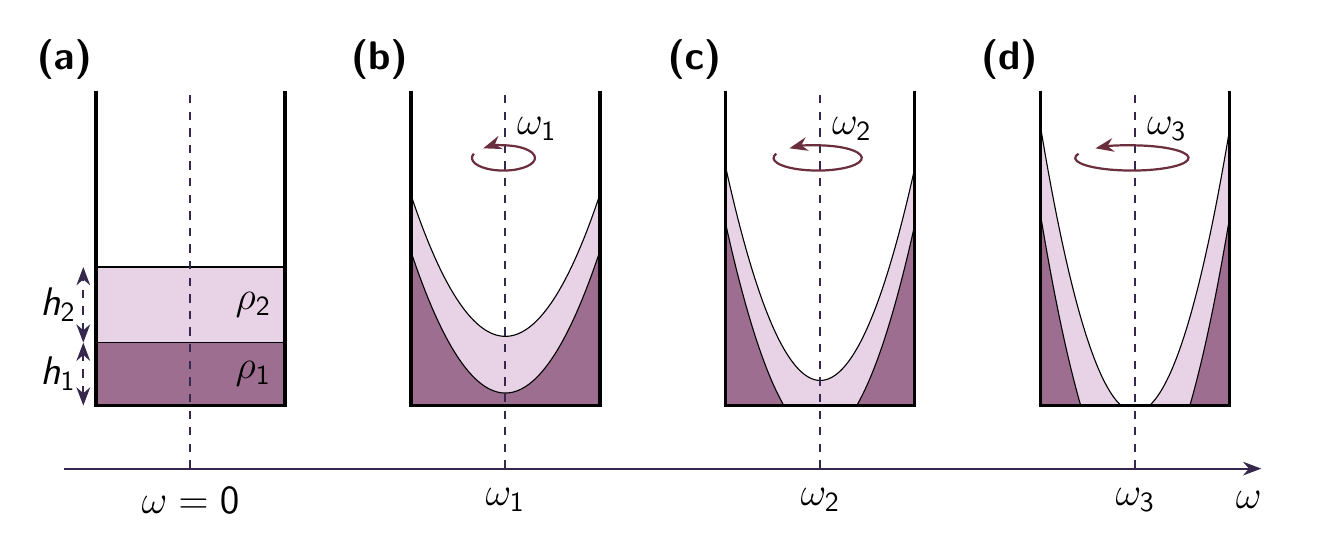
\begin{tikzpicture}[scale=0.8]
    %%Background
    \draw[draw=none] (0,-1) to (20,7);

    %% Initial state
    \draw[fill=Liquid1] (1,1) rectangle (4,2);
    \draw[fill=Liquid2] (1,2) rectangle (4,3.2);
    \draw[very thick] (1,6) to (1,1) to (4,1) to (4,6);

    %% Low-speed rotating cup
    \draw[fill = Liquid2, domain=-1.5:1.5, samples = 200, smooth, variable=\t] 
    plot ({7.5+\t}, {2.1+\t*\t}) to (9,1) to (6,1);
    \draw[fill = Liquid1, domain=-1.5:1.5, samples = 100, smooth, variable=\t] 
    plot ({7.5+\t}, {1.2+\t*\t}) to (9,1) to (6,1);
    
    \draw[very thick] (6,6) to (6,1) to (9,1) to (9,6);


    %% Medium-speed rotating cup
    \draw[fill = Liquid2, domain=-1.5:1.5, samples = 200, smooth, variable=\t] 
    plot ({12.5+\t}, {1.4+1.5*\t*\t}) to (14,1) to (11,1);
    \draw[fill = Liquid1, domain=-1.5:1.5, samples = 100, smooth, variable=\t] 
    plot ({12.5+\t}, {0.5+1.5*\t*\t}) to (14,1) to (11,1);
    \draw[draw=none, fill=white] (11,1) rectangle (14,0.2);
    
    \draw[very thick] (11,6) to (11,1) to (14,1) to (14,6);

    %% High-speed rotating cup
    \draw[fill = Liquid2, domain=-1.5:1.5, samples = 200, smooth, variable=\t] 
    plot ({17.5+\t}, {0.9+2*\t*\t}) to (19,1) to (16,1);
    \draw[fill = Liquid1, domain=-1.5:1.5, samples = 100, smooth, variable=\t] 
    plot ({17.5+\t}, {-0.5+2*\t*\t}) to (19,1) to (16,1);
    \draw[draw=none, fill=white] (16,1) rectangle (19,-1);
    
    \draw[very thick] (16,6) to (16,1) to (19,1) to (19,6);

    %% Note
    \draw[Note, thick, -Stealth] (0.5,0) to (19.5,0);
    \draw[Note, thick, dashed]
    (2.5,0) to (2.5,6)
    (7.5,0) to (7.5,6)
    (12.5,0) to (12.5,6)
    (17.5,0) to (17.5,6)
    ;

    \draw
    (2.5,-0.5) node{\Large\(\omega=0\)}
    (7.5,-0.5) node{\Large\(\omega_1\)}
    (12.5,-0.5) node{\Large\(\omega_2\)}
    (17.5,-0.5) node{\Large\(\omega_3\)}
    (19.3,-0.5) node{\Large\(\omega\)}
    (8,5.4) node{\Large\(\omega_1\)}
    (13,5.4) node{\Large\(\omega_2\)}
    (18,5.4) node{\Large\(\omega_3\)}
    ;

    \draw[Rotate, thick, -Stealth] (7,5) arc[start angle=-200, end angle=130, x radius=0.5, y radius=0.2];
    \draw[Rotate, thick, -Stealth] (11.8,5) arc[start angle=-200, end angle=130, x radius=0.7, y radius=0.2];
    \draw[Rotate, thick, -Stealth] (16.6,5) arc[start angle=-200, end angle=130, x radius=0.9, y radius=0.2];
    
    \draw[Note, thick, dashed, Stealth-Stealth] (0.8,1) to (0.8,2);
    \draw[Note, thick, dashed, Stealth-Stealth] (0.8,2) to (0.8,3.2);
    \draw
    (0.4,1.5) node{\Large\(h_1\)}
    (0.4,2.6) node{\Large\(h_2\)}
    (3.5,1.5) node{\Large\(\rho_1\)}
    (3.5,2.6) node{\Large\(\rho_2\)}
    ;
    
    \draw
    (0.5,6.5) node{\Large\textbf{(a)}}
    (5.5,6.5) node{\Large\textbf{(b)}}
    (10.5,6.5) node{\Large\textbf{(c)}}
    (15.5,6.5) node{\Large\textbf{(d)}}
    ;

    
\end{tikzpicture}

\end{document}
